\documentclass{book}

\usepackage{geometry}
\usepackage[utf8]{inputenc}
\usepackage{amsmath}
\usepackage{amsfonts}
\usepackage{amssymb}
\usepackage{graphicx}
\usepackage[utf8]{inputenc}
\usepackage{amsmath}
\usepackage{amsfonts}
\usepackage{amssymb}
\usepackage{listings}
\usepackage{xcolor}
\usepackage[most]{tcolorbox}
\usepackage{mathtools}
\usepackage[colorlinks=false, linktocpage=true]{hyperref}

\usepackage{booktabs}% http://ctan.org/pkg/booktabs
\newcommand{\tabitem}{~~\llap{\textbullet}~~}
\usepackage{longtable}
 
\usepackage{caption}
\DeclareCaptionType{code}[Code Listing][List of Code Listings] 

\definecolor{codegreen}{rgb}{0,0.6,0}
\definecolor{codegray}{rgb}{0.5,0.5,0.5}
\definecolor{codepurple}{rgb}{0.58,0,0.82}
\definecolor{backcolour}{rgb}{0.95,0.95,0.92}
 
\lstdefinestyle{mystyle}{
    backgroundcolor=\color{backcolour},   
    commentstyle=\color{codegreen},
    keywordstyle=\color{magenta},
    numberstyle=\tiny\color{codegray},
    stringstyle=\color{codepurple},
    basicstyle=\ttfamily\footnotesize,
    breakatwhitespace=false,         
    breaklines=true,                 
    captionpos=b,                    
    keepspaces=true,                 
    numbers=left,                    
    numbersep=5pt,                  
    showspaces=false,                
    showstringspaces=false,
    showtabs=false,                  
    tabsize=2
}
 
\lstset{style=mystyle}

\setlength{\parindent}{0em}
\setlength{\parskip}{1em}

\author{Brian Rashap, Ph.D.}
\title{PHYS 1320 - Calculus-based Physics II}

\geometry{letterpaper, portrait, margin=0.75in}

\begin{document}
\frontmatter

\maketitle


\mainmatter

\chapter{Module 1: Chapter 5 - Electric Charges and Fields}

From Newton's Second Laws of Mechanics:

\begin{equation}
F = ma
\end{equation}

A force can be recognized by the effect it has on an object. When studying gravitation, we examined the force of gravity that acts on all objects with mass. Similarly, the electric force acts on all objects with a property called charge. While gravity is an attractive force, the electric force can be either attractive or repulsive.  

\section{Section 5.1 Electric Charge}

The ancient Greek philosopher Thales of Miletus (624-546 BCE)recorded that when amber was vigorously rubbed with a piece of fur, it created a force that attracted them to each other. They also attracted other non-metallic objects even when not touched. 

\begin{figure}[h]
\begin{center}
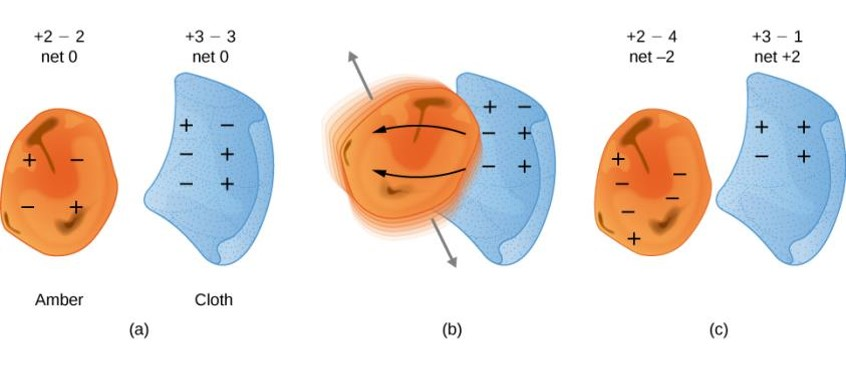
\includegraphics[scale=0.40]{fig/fig_05_05.jpg}
\caption{Materials rubbed together}
\label{fig:05_06}
\end{center}
\end{figure}

The English physicist William Gilbert (1544-1603) also studied attractive forces. He worked with a variety of substances. His findings included:
\begin{itemize}
\item Metals never exhibited this force, whereas minerals did
\item Two "electrified" amber rods would repel each other. 
\end{itemize}

This suggested that were two types of electric properties: attractive and repulsive. This property came to be known as Electric Charge. The force is repulsive between between the same type of charge and attractive between the charges are of opposite types. 

A Leyden jar (an early version of what is now called a capacitor) allowed experimenters to store large amounts of electric charge. Benjamin Franklin used such a jar to demonstrate that lightning behaved exactly like the electricity he got from the equipment in his laboratory.

\begin{figure}[h]
\begin{center}
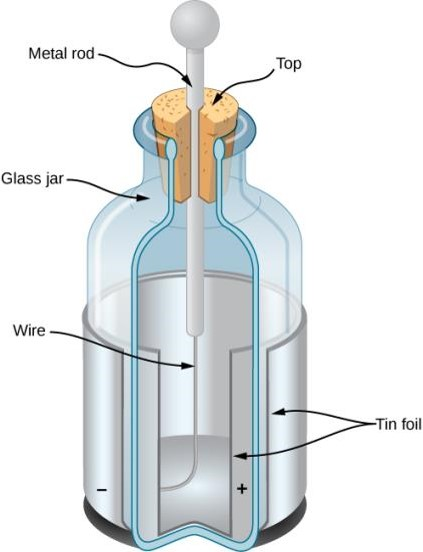
\includegraphics[scale=0.40]{fig/fig_05_06.jpg}
\caption{Leyden Jar}
\label{fig:05_06}
\end{center}
\end{figure}


\end{document}
